\documentclass[t]{beamer}

% Load general definitions
% Preamble file - general definitions, package loading, etc.

%=================================
% Load packages
\usepackage{amssymb,amsmath}
\usepackage{graphicx}
\usepackage{url}
\usepackage{tikz}
\usetikzlibrary{mindmap,trees,arrows}
\usepackage{fancyvrb}
\usepackage[english]{babel}
\usepackage[latin1]{inputenc}
\usepackage{subfigure}
\usepackage{times}
\usepackage[T1]{fontenc}
\usepackage{cancel}
\usepackage{color}
\usepackage{listings}

%=================================
% Set mode
\mode<presentation>
{
	\usetheme{Madrid}
	\usecolortheme{whale}
	\useoutertheme{infolines}
	\setbeamercovered{invisible}
}

% Get rid of nav bar
\beamertemplatenavigationsymbolsempty

% Insert frame number at bottom of the page.
\usefoottemplate{\hfil\tiny{\color{black!90}\insertframenumber}} 

%=================================
% Define new commands

\newcommand\Real{{\mathbb{R}}}
%\newcommand{\vi}{\vspace{0.6\baselineskip}}
%\newcommand{\goodgap}{\hspace{\subfigtopskip}\hspace{\subfigbottomskip}}


% Equation environments
\newcommand{\beq}{\begin{equation}}
\newcommand{\eq}{\end{equation}}
\newcommand{\beqs}{\begin{equation*}}
\newcommand{\eqs}{\end{equation*}}
\newcommand{\beqn}{\begin{eqnarray}}
\newcommand{\eqn}{\end{eqnarray}}

% Bold variables
\newcommand{\mbf}[1]{\ensuremath{\mathbf{#1}}}

% Itemization
\newcommand{\bitem}{\begin{itemize}}
\newcommand{\eitem}{\end{itemize}}
\newcommand{\spitem}{\vskip 1em\item}
\newcommand{\bitems}{\begin{itemize}\item}
\newcommand{\benums}{\begin{enumerate}\item}
\newcommand{\eenum}{\end{enumerate}}

% color blocks
\newenvironment{colorblock}[2]{%
\setbeamercolor{block title}{#2}
\begin{block}{#1}}{\end{block}}

% Vertical spacing
\newcommand{\vone}{\vskip 1em}
\newcommand{\vhalf}{\vskip .5em}

% Frame environments
\newenvironment{ftst}[3][t]{%
\begin{frame}{environment=ftst,#1}
\frametitle{#2}
\framesubtitle{#3}}{\end{frame}}

\newenvironment{ftstf}[2]{
\begin{frame}[fragile,environment=ftstf]
\frametitle{#1}
\framesubtitle{#2}}{\end{frame}}

% colors
\definecolor{MyGray}{rgb}{0.5,0.5,0.5}
\definecolor{MyDBGray}{rgb}{0.1,0.1,0.4}
\definecolor{darkgreen}{rgb}{0,0.4,0}
\definecolor{black}{rgb}{0,0,0}
\def\defn#1{{\color{red} #1}}

% Footnote
\renewcommand{\thefootnote}{\alph{footnote}}

% Relaxed footnotes
\newcommand{\lfr}[1]{\let\thefootnote\relax\footnote{\tiny #1}}

% Verbatim environment - using FANCYVRB package
\DefineVerbatimEnvironment%
{rcode}{Verbatim}
{fontsize=\scriptsize}

% Verbatim environment - using LISTINGS package
%\lstnewenvironment{rcode} {\lstset{	language = R,
%									basicstyle = \scriptsize\ttfamily,
%									showspaces = false,
%									showstringspaces = false,
%									showtabs = false,
%									keywordstyle = \color{black}\bfseries,
%									commentstyle = \color{darkgreen},
%									numbers = none,
%									otherkeywords={	<-,
%													ggplot,
%													geom_boxplot,
%													facet_grid,
%													shapiro.test,
%													fligner.test,
%													glht,
%													with},
%									deletekeywords={data,
%													model,
%													residuals,
%													c,
%													axis,
%													default,
%													labels,
%													qq.text}}}%
%{}


% Specific definitions
\title[]{Design and Analysis of Experiments}
\subtitle[]{05 - Statistical Inference}
\author[]{Felipe Campelo\\{\footnotesize http://www.cpdee.ufmg.br/\textasciitilde fcampelo}}
\institute{Graduate Program in Electrical Engineering}
\date{\scriptsize Belo Horizonte\\March 2015}

\begin{document}

% cover page
\setbeamertemplate{footline}{}
\begin{frame}
\begin{flushright}

\includegraphics[width=.25\textwidth]{../figs/principal_completa3_ufmg}
\end{flushright}
  \titlepage
  \begin{tikzpicture}[remember picture,overlay]
  \node[anchor=south east,xshift=-5pt,yshift=122pt] at (current page.south east) {\tiny Version 2.11};
  \node[anchor=south west,yshift=0pt] at (current page.south west) {
\includegraphics[width=.15\textwidth]{../figs/by-nc-sa.png}};
  \end{tikzpicture}  
\end{frame}

%=====

% quotation page
  \begin{frame}[b]
		\frametitle{}
\begin{columns}[T]
\column{0.79\textwidth}
\flushright{\small ``\textit{Chance is commonly viewed as a self-correcting process\\
in which a deviation in one direction induces a deviation\\
in the opposite direction to restore the equilibrium. In fact,\\
deviations are not ``corrected'' as a chance process unfolds,\\
they are merely diluted.}''\\\ \\
Amos Nathan Tversky\\
1937-1996\\
Israeli cognitive and mathematical psychologist\\}
\column{0.21\textwidth}
\begin{tikzpicture}[remember picture,overlay]
\node[anchor=south east,yshift=26pt,xshift=0pt] at (current page.south east)
{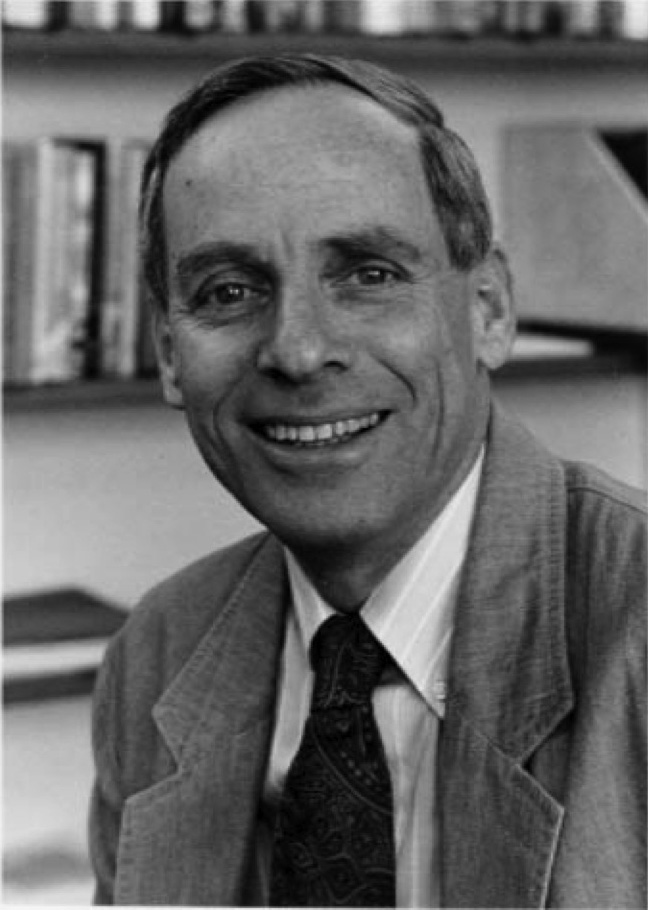
\includegraphics[width=\textwidth]{../figs/Tversky.jpg}};
\end{tikzpicture}
\end{columns}
\vhalf
\let\thefootnote\relax\footnote{\tiny Image: \url{http://upload.wikimedia.org/wikipedia/he/2/2b/Amos_Tversky.jpg}}
\end{frame}

%=====

% Main slides
\begin{ftst}
{Statistical Inference}
{Introduction}
Definitions such as point estimators and statistical intervals belong to a branch of statistical theory known as \textit{descriptive statistics}, that is, methods that are focused on accurately describing characteristics such as location or uncertainty about a given population parameter;
\vone
While these concepts are certainly important, in many cases description is not enough -- one may need decision-making tools to deal with information from random samples, tools that allow a researcher to perform \textit{inference} with a quantifiable degree of certainty.
\end{ftst}

%=====

\begin{ftst}
{Statistical hypotheses}
{Scientific Hypotheses}
A \textit{hypothesis} is a proposed explanation for an observable phenomenon.
\vone
Scientific hypotheses must satisfy (at least) two conditions:

\bitems Testability;
	\item Falsifiability;
\eitem
\vone
\begin{columns}[T]
    \column{0.75\textwidth}
	\begin{colorblock}{}{bg=green!30,fg=black}
	``\textit{The more we learn about the world, and the deeper\\
	our learning, the more conscious, specific,\\
	and articulate will be our knowledge of what\\
	we do not know, our knowledge of our ignorance.}''\\
	\flushright\vspace{-1em}\small Sir Karl R. Popper\\
	\flushright\vspace{-1em}\small (1902-1994)\\
	\flushright\vspace{-1em}\small Austro-British philosopher
	\end{colorblock}
	\column{0.25\textwidth}
\begin{tikzpicture}[remember picture,overlay]
\node[anchor=south east,yshift=13pt,xshift=0pt] at (current page.south east) {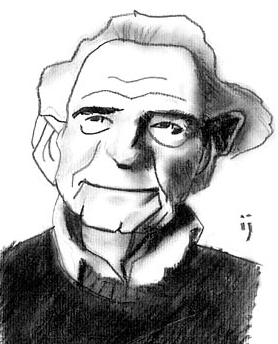
\includegraphics[width=\textwidth]{../figs/popper.png}};
%\node[anchor=south east,yshift=0pt,xshift=-15pt] at (current page.south east) {Karl Popper};
\end{tikzpicture}
\end{columns}
\let\thefootnote\relax\footnote{\tiny Image: Copyright 2008 Ivan Jer\^onimo \url{http://www.ivanjeronimo.com.br/imagem.php?imagem=30}}
\end{ftst}

%=====

\begin{ftst}
{Statistical Hypothesis}
{The hypothetico-deductive model}
The \textit{hypothetico-deductive model} of construction of scientific knowledge includes:

\bitems Formulation of falsifiable hypotheses;
	\item Refutation or corroboration of the hypotheses by the data;
	\item Comparison between alternative hypotheses - principle of parsimony (Ockham's razor);
	\item Predictive power;
\eitem

\begin{columns}[T]
	\column{0.20\textwidth}
\begin{tikzpicture}[remember picture,overlay]
\node[anchor=south west,yshift=20pt,xshift=15pt] at (current page.south west) {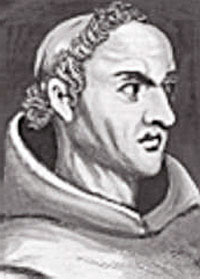
\includegraphics[width=.7\textwidth]{../figs/ockham2.png}};
\end{tikzpicture}
    \column{0.80\textwidth}
    \vhalf
	\begin{colorblock}{}{bg=green!30,fg=black}
	``\textit{Numquam ponenda est pluralitas sine necessitate.}''\\
	\flushright\vspace{-1em}\small William of Ockham\\
	\flushright\vspace{-1em}\small (1287-1347)\\
	\flushright\vspace{-1em}\small English philosopher and theologian\\
	\end{colorblock}
\end{columns}
\let\thefootnote\relax\footnote{\tiny Image: \url{http://www.philosophybasics.com/philosophers_ockham.html}}
\end{ftst}


%=====

\begin{ftst}
{Statistical Hypotheses}
{Definitions}
\textit{Statistical hypotheses} are defined as objective statements about parameters of one ore more populations;
\vone
\textbf{Attention}: the statements in statistical hypotheses are about parameters of the \textit{population} or \textit{model}, \textbf{not the \textit{sample}}.
\vone
On frequentist approaches, the formal test of hypotheses involves the contrast between \textit{null} and \textit{alternative} hypotheses.
\begin{columns}[T]
	\column{0.48\textwidth}
	\begin{block}{Null hypothesis ($H_0$)}
	\small
	\bitems Absence of effects;
	\item \textit{Conservative} model;
	\item Point value for the parameter.\eitem
	\textbf{Example:} $H_0: \mu = 25$
	\end{block}
	\column{0.48\textwidth}
	\begin{block}{Alternative hypothesis ($H_1$)}
	\small 
	\bitems Presence of some effect;
	\item Existence of something ``new''.
	\item Interval value for the parameter.\eitem
	\textbf{Example:} $H_1: \mu \neq 25$
		\end{block}
	\end{columns}
\end{ftst}

%=====

\begin{ftst}
{Statistical Hypotheses}
{Definitions}
Determination of the reference value for the null hypothesis $H_0$:

\bitems Previous knowledge about the process (investigation of changes);
	\item Value obtained from theory or models (model validation);
	\item Project requirements (investigation of system compliance);
\eitem
\vone
Hypothesis testing involves:

\bitems Obtaining the sample;
	\item Calculation of test statistics;
	\item Decision based on the computed value;
\eitem
\end{ftst}

%=====

\begin{ftst}
{Statistical Hypotheses}
{Example}
Suppose you are a large-scale customer of green peas\footnote[1]{\tiny We could use any other item on your usual grocery list, but why not pay a little tribute to Gregor Mendel?}, and that you want to determine if the $500$g packages from a given food supplier really contain their nominal weight (at least on average).
\vhalf
In this case the null hypothesis could be defined as:
\textit{the average net weight of a package is $500$g}, and the alternative of interest could be expressed as the complementary inequality.
\beqs\begin{cases}
H_0: \mu = 500g \\
H_1: \mu \neq 500g 
\end{cases}\eqs
\vone
Suppose still that $n=10$ randomly selected packs are obtained from this supplier, and their contents are weighted using a calibrated scale;
\begin{tikzpicture}[remember picture,overlay]
\node[anchor=north east,yshift=12pt,xshift=-5pt] at (current page.north east) {
\includegraphics[width=0.2\textwidth]{../figs/peas.png}};
\end{tikzpicture}
\let\thefootnote\relax\footnote{\tiny Image: \url{http://www.storko.eu/ed_files/image/green-peas.jpg}}
\end{ftst}

%=====

\begin{ftst}
{Statistical Hypotheses}
{Example}
Since the sample mean $\bar{x}$ is a good estimator of the real mean $\mu$, we can assume:

\bitems If $\bar{x} \cong 500$g - corroboration of $H_0$;
\item If $\bar{x} \ll 500$g or $\bar{x} \gg 500$g - refutation of $H_0$;
\eitem
\vone
Suggests the use of $\bar{x}$ as basis for a statistical test.
\vone
Definition of a \textit{critical region} for the rejection of $H_0$:
\vone\vhalf
\centering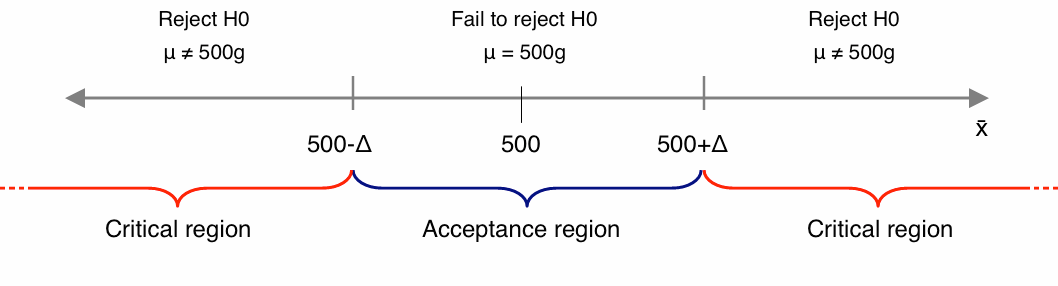
\includegraphics[width=\textwidth]{../figs/regcrit2.png}
\begin{tikzpicture}[remember picture,overlay]
\node[anchor=north east,yshift=12pt,xshift=-5pt] at (current page.north east) {
\includegraphics[width=0.2\textwidth]{../figs/peas.png}};
\end{tikzpicture}
\end{ftst}

%=====

\begin{ftst}
{Inferential Errors}
{Type I error}
\begin{colorblock}{}{bg=green!30,fg=black}
\textbf{Type I error} (false positive): rejecting the null hypothesis when it is true.
\end{colorblock}
\vone
The probability of occurrence of a false positive in any hypothesis testing procedure is generally known as the \textit{significance level} of the test, represented by Greek letter $\alpha$:
\beqs \alpha = P\left(\mbox{type I error}\right) = P\left(\mbox{reject }H_0|H_0\mbox{ is true}\right)\eqs
\vone
Another frequently used term is the \textit{confidence level} of the test, given by $(1-\alpha)$.
\end{ftst}

%=====

\begin{ftst}
{Inferential Errors}
{Type I error}
For a given sample, the selected value of $\alpha$ defines the critical threshold for the rejection of $H_0$.
\vone
If $H_0$ is true (i.e., if $\mu=500$g), the distribution of values of $\bar{x}$ is aproximately normal (remember the CLT), with average $500$ and variance given by $s^2/n$;
\vone
For a Type-I error probability $\alpha=0.05$, the critical values of the distribution of $\bar{x}$ are the ones for which the probability content within the acceptance region is $1-\alpha = 0.95$.
\begin{tikzpicture}[remember picture,overlay]
\node[anchor=south east,yshift=0pt,xshift=0pt] at (current page.south east) {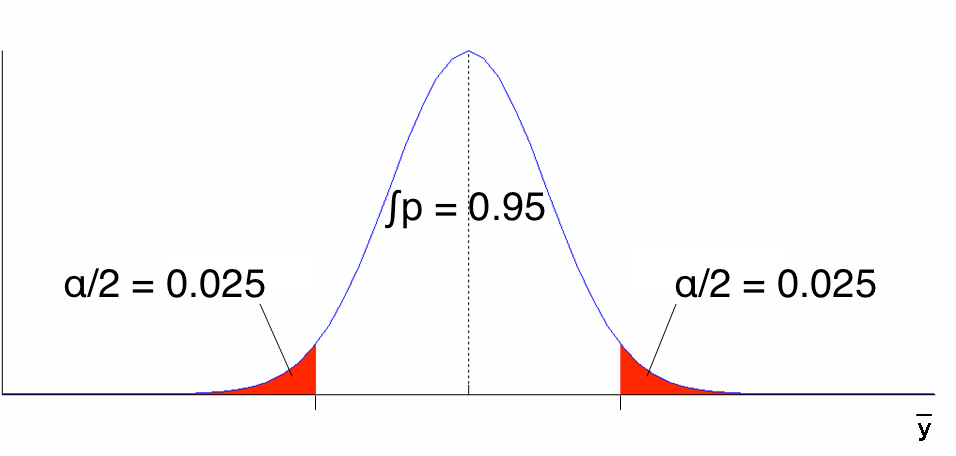
\includegraphics[width=0.5\textwidth]{../figs/alpha.png}};
\end{tikzpicture}
\end{ftst}

%=====

\begin{ftst}
{Inferential Errors}
{Type II error}
\begin{colorblock}{}{bg=green!30,fg=black}
\textbf{Type II error} (false negative): failure to reject the null hypothesis when it is false.
\end{colorblock}
\vone
The probability of occurrence of a false negative in any hypothesis testing procedure is generally represented by the Greek letter $\beta$:

\beqs 
\beta = P\left(\mbox{type II error}\right) = P\left(\mbox{not reject }H_0|H_0\mbox{ is false}\right)
\eqs

The quantity ($1-\beta$) is known as \textit{power} of the test, and quantifies its sensitivity to effects that violate the null hypothesis.
\end{ftst}

%=====

\begin{ftst}
{Inferential Errors}
{Type II error}
\begin{columns}[T]
	\column{0.55\textwidth}
		Unlike the Type-I error, the definition of the Type-II error rate requires further specification of the value of the parameter being investigated under the alternative hypothesis;
		\vone
		The probability of failing to reject a false $H_0$ is strongly dependent on the magnitude of the difference between the value under $H_0$ and the real value of the parameter.
	\column{0.45\textwidth}
	\end{columns}
\begin{tikzpicture}[remember picture,overlay]
\node[anchor=south east,yshift=130pt,xshift=-5pt] at (current page.south east) {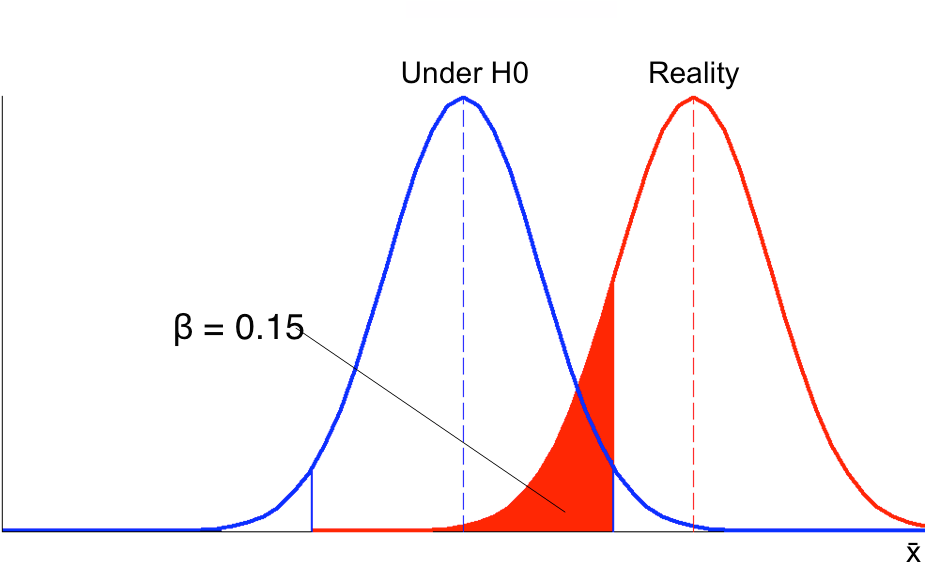
\includegraphics[width=0.45\textwidth]{../figs/beta-a.png}};
\node[anchor=south east,yshift=30pt,xshift=-5pt] at (current page.south east) {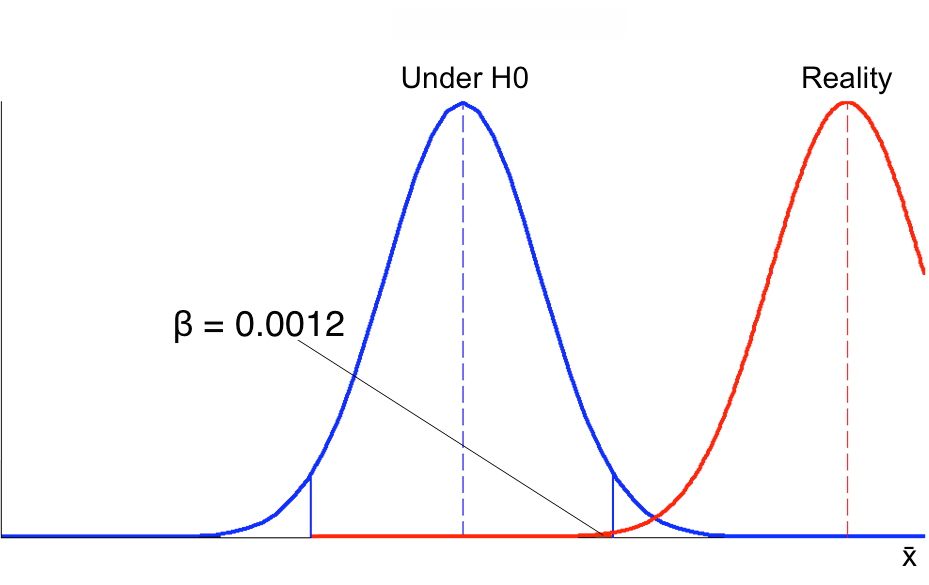
\includegraphics[width=0.45\textwidth]{../figs/beta-d.png}};
\end{tikzpicture}

\end{ftst}

%=====

\begin{ftst}
{Inferential Errors}
{Type II error}
The power of a test is governed by several factors:

\bitems Controllable: significance level, sample size;
	\item Uncontrollable: real value of the parameter;
\eitem

If $H_0$ is false, the smaller the magnitude of the difference between the real value of the parameter and the one under the null hypothesis, the greater the probability of a type II error - \textbf{\textit{but the practical importance of the effect gets smaller}}.
\end{ftst}

%=====

\begin{ftst}
{Inferential Errors}
{Considerations}
\textbf{Type I error} ($\alpha$) depends only on the distribution of the null hypothesis - easier to control;
\vone
\textbf{Type II error} ($\beta$) depends on the real value of the parameter - more difficult to specify and control;
\vone
These characteristics lead to the following classification of the conclusions obtained from the test of hypotheses:
\begin{block}{}
\bitems Rejection of $H_0$ - \textit{strong} conclusion; 
\spitem Failure to reject $H_0$ - \textit{weak} conclusion (but we can strengthen it);
\eitem
\end{block}
\vone
It is important to remember that failing to reject $H_0$ does not mean that there is evidence in favor of $H_0$ - it only suggests that it is a better model than the alternative.
\end{ftst}

%=====

\begin{ftst}
{Hypothesis Testing}
{General procedure}
\bitems Identify the parameter of interest;
	\item Define $H_0$ and $H_1$ (one- or two-sided);
	\item Determine desired $\alpha$, $\beta$;
	\item Define minimally interesting effect $\delta^*$;
	\item Calculate sample size;
	\item Determine the test statistic and critical region;
	\item Compute the statistic;
	\item Decide whether or not to reject $H_0$;
\eitem

\begin{tikzpicture}[remember picture,overlay]
\node[anchor=south east,yshift=2pt, xshift=-15pt] at (current page.south east) {\includegraphics[width=.21\textwidth]{../figs/hypothesis-wine.png}};
\end{tikzpicture}
\let\thefootnote\relax\footnote{\tiny Image (c) Roots Run Deep Winery: \url{http://www.rootsrundeep.com/hypothesis.html}}
\end{ftst}

%=====

\begin{ftst}
{Hypothesis Testing}
{Mean of a normal distribution, variance known}
Back to the green peas example, we want to determine if there is any significant deviation on the mean weight of the packages. Assume for now that the variance of the process is known. The test hypotheses are defined as:

\beqs\begin{cases}
H_0: \mu = 500g\\
H_1: \mu \neq 500g
\end{cases}\eqs
\vone
Let the desired significance level be $\alpha = 0.05$;
\vone
Given these characteristics, we expect that the sampling distribution of $\bar{X}$ is normal, with variance $Var(\bar{X})=\sigma^2/n$ and, if $H_0$ is true -- mean $\mu_{\bar{X}}=\mu_0=500$;
\begin{tikzpicture}[remember picture,overlay]
\node[anchor=north east,yshift=12pt,xshift=-5pt] at (current page.north east) {
\includegraphics[width=0.2\textwidth]{../figs/peas.png}};
\end{tikzpicture}
\end{ftst}

%=====

\begin{ftst}
{Hypothesis Testing}
{Mean of a normal distribution, variance known}
Based on these characteristics, the variable
\beqs Z_0 = \frac{\bar{X} - \mu_0}{\sigma/\sqrt{n}}\eqs
\vhalf
\noindent will be distributed according to the standard normal, $\mathcal{N}\left(0,1\right)$, but only \textbf{if $H_0$ is true}.
\vone
This result implies a probability of $\left(1-\alpha\right)$ that $Z_0$ will fall within the range $(\pm z_{\alpha/2})$\footnote[2]{\tiny $z_{\alpha/2}$ is the superior $100(1-\alpha/2)\%$ percentile of the standard normal distribution;} if $H_0$ is true, which provides a selection criterion between $H_0$ and $H_1$:

\bitems If $|z_0|>z_{\alpha/2}$, we reject $H_0$ at the confidence level $1-\alpha$;
	\item Otherwise, there is not enough evidence to reject $H_0$;
\eitem
\begin{tikzpicture}[remember picture,overlay]
\node[anchor=north east,yshift=12pt,xshift=-5pt] at (current page.north east) {
\includegraphics[width=0.2\textwidth]{../figs/peas.png}};
\end{tikzpicture}
\end{ftst}

%=====

\begin{ftst}
{Hypothesis Testing}
{Mean of a normal distribution, variance known}
Assume that we got $\bar{x} = 496.48 g$ from our $n=10$ observations, and that $\sigma = 10g$. In this case,

\beqs 
z_0 = \frac{496.48 - 500}{10/\sqrt{10}} = -1.113
\eqs
\vhalf
The critical values of the standard normal distribution are $\pm z_{\alpha/2} = \pm z_{0.025} = \pm 1.96$;
\vone
Since $|z_0|<z_{0.025}$, we can conclude that there is not enough evidence to reject $H_0$ at the $95\%$ confidence level.
\begin{tikzpicture}[remember picture,overlay]
\node[anchor=north east,yshift=12pt,xshift=-5pt] at (current page.north east) {
\includegraphics[width=0.2\textwidth]{../figs/peas.png}};
\end{tikzpicture}
\end{ftst}

%=====

\begin{ftstf}
{Hypothesis Testing}
{Mean of a normal distribution, variance known}

\begin{rcode}
> if(!require(TeachingDemos)){
+ 	install.packages("TeachingDemos")
+ 	library(TeachingDemos)
+ }
> 
> sample<-scan("../data files/greenpeas.txt")
> z.test(as.numeric(sample),
+        mu=500,
+        stdev=10)

One Sample z-test
data:  as.numeric(sample)
z = -1.1131, n = 10.000, Std. Dev. = 10.000, 
Std. Dev. of the sample mean = 3.162, 
p-value = 0.2657
alternative hypothesis: true mean is not equal to 500
95 percent confidence interval:
 490.282 502.678
sample estimates:
mean of as.numeric(sample) 
                    496.48 
\end{rcode}
\begin{tikzpicture}[remember picture,overlay]
\node[anchor=north east,yshift=-60pt,xshift=-5pt] at (current page.north east) {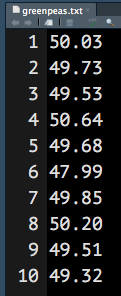
\includegraphics[width=0.22\textwidth]{../figs/peastxt.png}};
\node[anchor=north east,yshift=12pt,xshift=-5pt] at (current page.north east) {
\includegraphics[width=0.2\textwidth]{../figs/peas.png}};
\end{tikzpicture}
\end{ftstf}

%=====

\begin{ftst}
{Hypothesis Testing}
{Mean of a normal distribution, variance unknown}
Suppose now a more realistic situation in which the real variance is unknown. Besides, assume that we are interested in detecting only negative deviations from the nominal contents of the package.
\vone
The test hypotheses can be defined as:
\beqs\begin{cases}
H_0: \mu = 500g\\
H_1: \mu < 500g 
\end{cases}\eqs
\vhalf
In this second scenario we want to be more conservative, so we pick a significance level of $\alpha = 0.01$;
\vone
It can be shown that, if \textbf{if $H_0$ is true}, then
\beqs T_0 = \frac{\bar{X} - \mu_0}{S/\sqrt{n}} \sim t_{n-1}
\eqs
\begin{tikzpicture}[remember picture,overlay]
\node[anchor=north east,yshift=12pt,xshift=-5pt] at (current page.north east) {
\includegraphics[width=0.2\textwidth]{../figs/peas.png}};
\end{tikzpicture}
\end{ftst}

%=====

\begin{ftst}
{Hypothesis Testing}
{Mean of a normal distribution, variance unknown}
From the same data, $\bar{x} = 496.48 g$, $n=10$, $s = 6.97 g$:
\beqs t_0 = \frac{496.48 - 500}{6.97/\sqrt{10}} = -1.5969\eqs
\vhalf
The critical value of this test statistic for the desired significance is $-t_{\alpha,n-1} = -t_{0.01,9} = -2.54$;
\vone
Given that $t_0 > -2.54$, we conclude that the evidence is insufficient to reject $H_0$ at the $99\%$ confidence level;
\begin{tikzpicture}[remember picture,overlay]
\node[anchor=north east,yshift=12pt,xshift=-5pt] at (current page.north east) {
\includegraphics[width=0.2\textwidth]{../figs/peas.png}};
\end{tikzpicture}
\end{ftst}

%=====

\begin{ftstf}
{Hypothesis Testing}
{Mean of a normal distribution, variance unknown}
\begin{rcode}
> t.test(sample,
+        alternative = "less",
+        mu = 500,
+        conf.level = 0.99)

	One Sample t-test
data:  sample
t = -1.5969, df = 9, p-value =0.07237
alternative hypothesis: true mean is less than 500
99 percent confidence interval:
     -Inf 502.6991
sample estimates:
mean of x 
   496.48
\end{rcode}
\begin{tikzpicture}[remember picture,overlay]
\node[anchor=north east,yshift=12pt,xshift=-5pt] at (current page.north east) {
\includegraphics[width=0.2\textwidth]{../figs/peas.png}};
\end{tikzpicture}
\end{ftstf}

%=====

\begin{ftst}
{Hypothesis Testing}
{Reporting results}
Description of the results:
\vone
\begin{block}{}
\centering\textit{(In)Sufficient evidence for rejecting $H_0$\\at the significance level $\alpha$.}
\end{block}
\vone
Even thought it is correct, this description is relatively poor:

\bitems It does not provide information on the intensity of the evidence for rejection/non-rejection;
	\item It imposes a predetermined significance level to the consumer of the information;
	\item Does not provide information the magnitude of the effect found or the sensitivity of the test.
\eitem
\end{ftst}

%=====

\begin{ftst}
{Hypothesis Testing}
{The p-value}
\begin{colorblock}{}{bg=green!30,fg=black}
\centering\textbf{p-value}: \textit{the lowest significance level that would lead\\to the rejection of $H_0$for the available data.}
\end{colorblock}
\vone
Can be interpreted as the probability under $H_0$ of the test statistic assuming a value at least as extreme as the one obtained;
\vone\vhalf
For the previous example, the p-value could be calculated as:
\beqs
p = P(t_0\leq -1.597|H_0 = \mbf{TRUE}) = \int\limits_{-\infty}^{-1.597}(t_{9})dt = 0.07237
\eqs
\vhalf

\begin{block}{}
\centering\textit{A priori} definition of the significance level is still important!
\end{block}
\end{ftst}

%=====

\begin{ftst}
{Hypothesis Testing}
{p-values, significance and effect sizes}
Statistical $\times$ practical significance: p-values can be made arbitrarily small, if $n$ is big enough;
\vone 
As an example, suppose a test of $H_0: \mu=500g$ against a two-sided alternative, with $n=5000, \bar{x}=499g,\ s=5g$. In this case we would have:

\bitems $t_0 = -14.142$;
\item $p = 1.02\times 10^{-23}$;\eitem
\vone	
Is it really \textit{that} significant?
\end{ftst}

%=====

\begin{ftst}
{Hypothesis Testing}
{p-values, significance and effect sizes}
To ``tell the whole story'' of the experiment, it is necessary to use \textbf{effect size estimators} alongside the tests of statistical significance; 
\vone
While there are whole books on the subject \footnote[3]{\tiny See, for instance, Paul D. Ellis' \textit{The Essential Guide to Effect Sizes}, Cambridge University Press, 2010.}, the main idea is quite simple - to quantify the magnitude of the observed deviation from the null hypothesis.
\vone
Examples of effect size estimators include the simple point estimator for the difference $\bar{x} - \mu_0$, or the dimensionless \textit{d} estimator:

\beqs
d = \frac{\bar{x}-\mu_0}{s}
\eqs

\noindent which quantifies the difference in terms of sample standard deviations.
\vone
\end{ftst}

%=====

\begin{ftstf}
{Hypothesis Testing}
{p-values, effects sizes and confidence intervals}
\begin{block}{}
\centering\textit{Point estimators + confidence intervals quantify the magnitude and accuracy of effects, and must be reported alongside the results of significance testing whenever possible.}
\end{block}
\vhalf
Suppose we are testing $H_0: \mu=500$ against the two-sided alternative hypothesis, with $n=10$ and $\alpha=0.01$. Assume that the population is known to be normal, with unknown variance. We'll use the same data as before:
\vhalf
\begin{rcode}
> t.test(sample, mu = 500, conf.level = 0.99)
(...)
t = -1.5969, df = 9, p-value = 0.1447
alternative hypothesis: true mean is not equal to 500
99 percent confidence interval:
 489.3166 503.6434
sample estimates:
mean of x 
   496.48 
\end{rcode}
\begin{tikzpicture}[remember picture,overlay]
\node[anchor=north east,yshift=12pt,xshift=-5pt] at (current page.north east) {
\includegraphics[width=0.2\textwidth]{../figs/peas.png}};
\end{tikzpicture}
\end{ftstf}

%=====

\begin{ftst}{Sample size and Type-II error}
{Some considerations}
The probability of Type-II error can be easily evaluated \textit{a posteriori}, but its definition \textit{a priori} requires some care;
\vone
The power of a test is essentially a function of 4 elements:
\bitems Actual size of the difference;
	\item Variability of the observations;
	\item Significance level;
	\item Sample size.
\eitem
\vone
The experimenter generally have little control over the first two.
\end{ftst}

%=====

\begin{ftst}{Sample size and Type-II error}
{Some considerations}
A strategy for estimating an effective lower bound for the power of a test includes a definition of an \textit{minimally interesting effect} $\delta^*$. 
\vone
This value must be derived from technical and scientific knowledge about the phenomenon or system under experimentation. 
\vhalf
\begin{block}{}
\centering It is essential to have a good understanding of the field in which the experiment will be conducted.
\end{block}
\vhalf
Once $\delta^*$ is defined, the experimenter can obtain an estimate of the variability of observations (e.g., by a pilot study), which can then be used to obtain an approximate power value for the experiment;
\end{ftst}

%=====

\begin{ftst}
{Sample size and Type-II error}
{Some considerations}
Having obtained this estimation of the Type-II error probability, one can run his/her experiment with a better understanding of its ability to detect effects of interest.
\vone
The test will have lower power for differences smaller than $\delta^*$, but these differences are below the minimally interesting effect; any effect greater than $\delta^*$ will result in a higher power for the test;
\vone
This technique can also be used as a way to compute the maximum necessary sample size for the experiment.
\end{ftst}

%=====

\begin{ftstf}
{Sample size and Type-II error}
{Example}
Suppose that on the green peas example one is really interested in detecting deviations from the nominal value greater than $1\%$, i.e., $\delta^* = 0.01*500 = 5g$. The researcher defines that, for this minimally interesting effect, a test power of $0.85$ is desired. The test will again be performed with $\alpha = 0.01$.
\vone
The same sample of $n=10$ packs is used. The estimated standard deviation for this sample is $s=6.97g$. From this data, we can compute the power of this test as:
\begin{columns}
\column[T]{0.5\textwidth}
\begin{rcode}
> s<-sqrt(var(sample))
> power.t.test(n=10, 
+        delta=5, 
+        sd=s, 
+        sig.level=0.01, 
+        type = "one.sample", 
+        alternative = "one.sided")
\end{rcode}
\column[T]{0.5\textwidth}
\begin{rcode}
One-sample t test power calculation 
n = 10
delta = 5
sd = 6.970382
sig.level = 0.01
power = 0.3474724
alternative = one.sided
\end{rcode}
\end{columns}
\begin{tikzpicture}[remember picture,overlay]
\node[anchor=north east,yshift=12pt,xshift=-5pt] at (current page.north east) {
\includegraphics[width=0.2\textwidth]{../figs/peas.png}};
\node[anchor=south east,yshift=30pt,xshift=-48pt] at (current page.south east) {\footnotesize\color{red}$\mbf{\longleftarrow}$ \textbf{Power}};
\end{tikzpicture}
\end{ftstf}

%=====

\begin{ftstf}
{Sample size and Type-II error}
{Example}
What is the smallest sample size needed to obtain the desired power of $0.85$?
\vhalf
\begin{rcode}
> power.t.test(power=0.85, delta=5, sd=s, sig.level=0.01,
               type = "one.sample", alternative = "one.sided")

One-sample t test power calculation 
n = 24.76091
delta = 5
sd = 6.970382
sig.level = 0.01
power = 0.85
alternative = one.sided
\end{rcode}
\vhalf
We need at least 25 observations to detect a $-5g\ (1\%)$ or larger deviation on the mean weight of the green peas packages with a power level of $0.85$.
\begin{tikzpicture}[remember picture,overlay]
\node[anchor=north east,yshift=12pt,xshift=-5pt] at (current page.north east) {
\includegraphics[width=0.2\textwidth]{../figs/peas.png}};
\node[anchor=south east,yshift=140pt,xshift=-182pt] at (current page.south east) {\footnotesize\color{red}$\mbf{\longleftarrow}$ \textbf{(round this value up)}};
\end{tikzpicture}
\end{ftstf}

\begin{ftst}
{Model validation}
{The normality assumption}
The assumption of normality, required for the \textbf{z} and \textbf{t} tests, needs to be validated.
\vhalf
\bitems Graphical/qualitative tests;
	\spitem Analytical/quantitative tests; 
\eitem
\vhalf
It is interesting to use both whenever possible.
\end{ftst}

%=====

\begin{ftstf}
{Model validation}
{The normality assumption}
Graphical/qualitative tests;
\vone
\begin{rcode}
> qqnorm(sample,
+        pch=16, cex=2)
> qqline(sample,
+        lty=2, lwd=2)
\end{rcode}
\begin{tikzpicture}[remember picture,overlay]
\node[anchor=south east,yshift=-10pt,xshift=10pt] at (current page.south east) {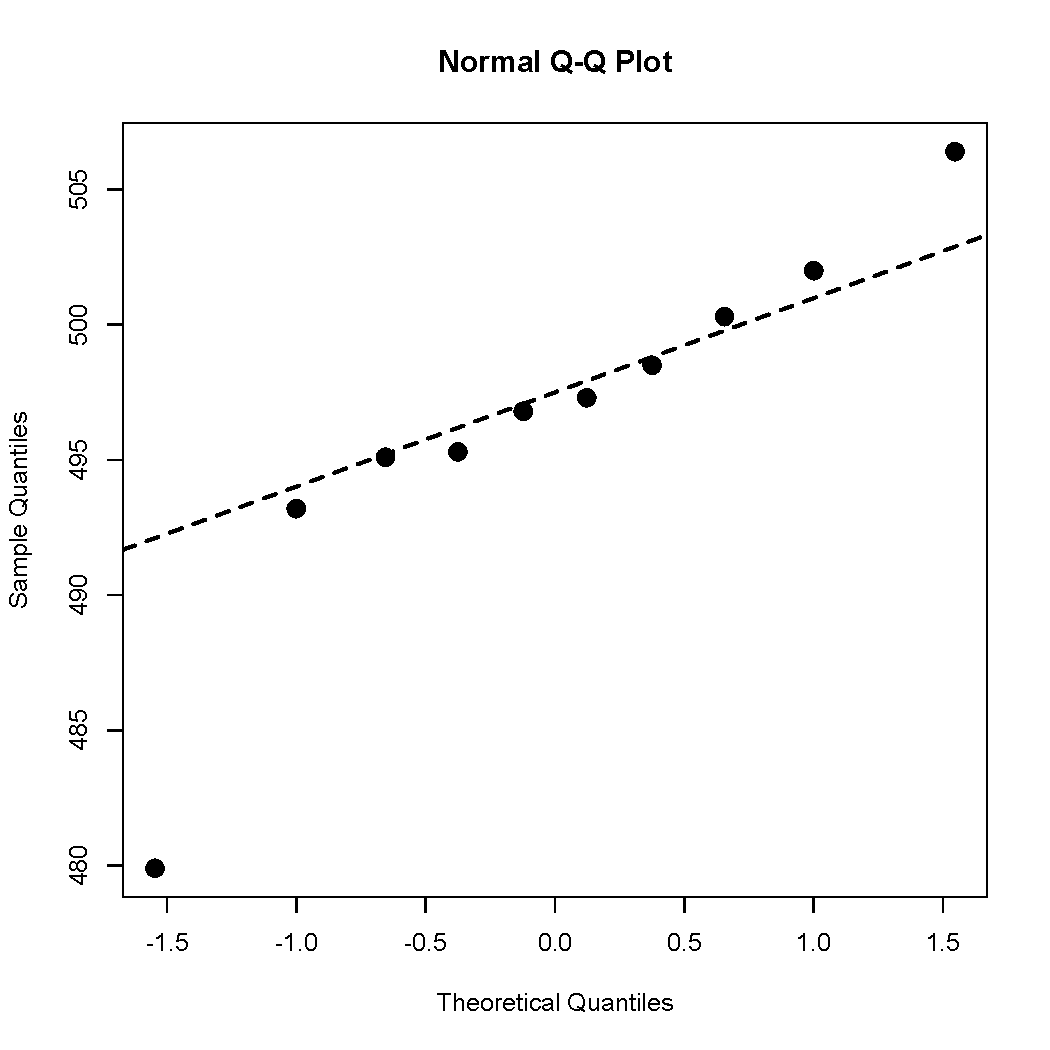
\includegraphics[width=.7\textwidth]{../figs/GraphNorm.pdf}};
\node[anchor=south east,yshift=28pt,xshift=-128pt] at (current page.south east) {\color{red}$\longleftarrow$ \textit{outlier}?};
\node[anchor=north east,yshift=12pt,xshift=-5pt] at (current page.north east) {
\includegraphics[width=0.2\textwidth]{../figs/peas.png}};
\end{tikzpicture}
\end{ftstf}

%=====

\begin{ftst}
{Model validation}
{The normality assumption}
There is a great variety of analytical tests of normality;
\bitems Shapiro-Wilk;
	\item Anderson-Darling;
	\item Lilliefors / Kolmogorov-Smirnov;
\eitem
\vone
These procedures use different aspects of the sample distribution to test the following hypotheses:
\beqs\begin{cases}
	H_0: \mbox{population is normal}\\
	H_1: \mbox{population is not normal}
\end{cases}\eqs
\vhalf
In this case, rejection of the null hypothesis suggests evidence that the sample came from a non-normal population. Generally we will use a low $\alpha$ (e.g., $0.01$) for these tests, and will consider their results together with a graphical analysis.
\end{ftst}

%=====

\begin{ftstf}
{Model validation}
{The normality assumption}
Even thought the Lilliefors test is possibly the most widely used for normality testing, the Shapiro-Wilk test tends to be more sensitive and has some other  interesting properties, so we will be using it throughout the course.
\vhalf
\begin{rcode}
> shapiro.test(sample)

Shapiro-Wilk normality test
data:  sample
W = 0.8809, p-value = 0.1335
\end{rcode}
\begin{tikzpicture}[remember picture,overlay]
\node[anchor=north east,yshift=12pt,xshift=-5pt] at (current page.north east) {
\includegraphics[width=0.2\textwidth]{../figs/peas.png}};
\end{tikzpicture}
\end{ftstf}

%=====

\begin{ftstf}
{Model validation}
{The independence assumption}
Another assumption of the statistical model used for the t-test is the independence of the residuals, that is, the absence of external (unmodeled) biases contaminating the data.
\vhalf
While there is no procedure to test independence in the general case, the Durbin-Watson test can be used to evaluate serial autocorrelations in the residual data, which can be useful to investigate contamination by order-dependent effects.
\begin{rcode}
> library(lmtest)
> dwtest(sample~1)

Durbin-Watson test
data:  sample ~ 1
DW = 2.1117, p-value = 0.573
alternative hypothesis: true autocorrelation is greater than 0
\end{rcode}
\begin{tikzpicture}[remember picture,overlay]
\node[anchor=north east,yshift=12pt,xshift=-5pt] at (current page.north east) {
\includegraphics[width=0.2\textwidth]{../figs/peas.png}};
\end{tikzpicture}
\end{ftstf}

%=====

\begin{ftstf}
{Model validation}
{The independence assumption}
As a test of serial autocorrelation, the Durbin-Watson test depends on the ordering of the data, so observations should be ordered (either in the data file or by manipulating the data vector) according to covariates that are suspected to introduce dependencies, e.g., order of collection, placement criteria, etc.
\vone
Violations of the independence assumption tend to be the hardest to deal with during the analysis, so extra care is recommended in the design of the experiment in order to prevent, control, or at least document all variables that could introduce dependencies in the data.
\end{ftstf}

%=====

\begin{ftst}
{The green peas experiment}
{Going over the process}
After examining the green peas example, it is interesting to go back and follow the recommended sequence for this kind of experiment:

\bitems Formulate question of interest;
	\spitem Define minimally interesting effect;
	\spitem Define desired confidence and power;
	\spitem Calculate required sample size;
	\spitem Collect data;
	\spitem Perform statistical analysis;
	\spitem Draw conclusions and recommendations.
\eitem
\begin{tikzpicture}[remember picture,overlay]
\node[anchor=north east,yshift=12pt,xshift=-5pt] at (current page.north east) {
\includegraphics[width=0.2\textwidth]{../figs/peas.png}};
\end{tikzpicture}
\end{ftst}

%=====


\begin{ftst}
{Bibliography}
{\ }
\scriptsize
\textbf{Required reading}

\benums D.C. Montgomery, G.C. Runger, \textit{Applied Statistics and Probability for Engineers}, Ch. 9.\\5th ed., Wiley, 2010. 
\item W. Thalheimer and S. Cook, \textit{How to calculate effect sizes from published research articles: A simplified methodology} - {\tiny\url{http://goo.gl/c0g1oK}}
\eenum

\textbf{Recommended reading}

\benums A. Reinhart, \textit{Statistics Done Wrong: the woefully complete guide} - {\tiny\url{http://www.statisticsdonewrong.com}}
\item S. Okasha, \textit{Philosophy of Science: A Very Short Introduction}, Oxford University Press, 2002.
\eenum
\end{ftst}

%=====

\begin{ftstf}{About this material}{Conditions of use and referencing}
\centering\footnotesize This work is licensed under the Creative Commons CC BY-NC-SA 4.0 license\\(Attribution Non-Commercial Share Alike International License version 4.0).\\
\vhalf
\url{http://creativecommons.org/licenses/by-nc-sa/4.0/}\\
\vone
\footnotesize Please reference this work as:\\
\footnotesize \flushleft Felipe Campelo (2015), \textit{Lecture Notes on Design and Analysis of Experiments}.\\Online: {\scriptsize\url{https://github.com/fcampelo/Design-and-Analysis-of-Experiments}}\\
Version 2.11, Chapter 5; Creative Commons BY-NC-SA 4.0.\\

\begin{Verbatim}[fontsize=\tiny]
    @Misc{Campelo2015-01,
      title={Lecture Notes on Design and Analysis of Experiments},
      author={Felipe Campelo},
      howPublished={\url{https://github.com/fcampelo/Design-and-Analysis-of-Experiments}},
      year={2015},
      note={Version 2.11, Chapter 5; Creative Commons BY-NC-SA 4.0.},
    }
\end{Verbatim}

\begin{tikzpicture} [remember picture,overlay]
\node[anchor=south,yshift=0pt] at (current page.south){ \includegraphics[width=.2\textwidth]{../figs/CCSomerights.png}};
\end{tikzpicture}
\end{ftstf}


\end{document}